\documentclass[a4paper,12pt]{report}
\usepackage[utf8]{inputenc}
\usepackage[francais]{babel}
\usepackage{fancyhdr}
\usepackage{graphicx}
\usepackage{tikz}
\usetikzlibrary{calc}
\usepackage{listings}
\usepackage{xcolor}
\definecolor{grey}{rgb}{0.9,0.9,0.9}
\usepackage{titlesec}
\usepackage{verbatim}
\usepackage{listings}
\usepackage{textcomp}
\usepackage{hyperref}
\usepackage{ amssymb }


\frenchbsetup{StandardLists=true}
\newcommand{\marge}{18mm}
\usepackage[left=\marge,right=\marge,top=\marge,bottom=\marge]{geometry}
\pagestyle{fancy}
\setlength{\headheight}{14pt}
\chead{
  \textbf{Nom :} Douaille
  \hspace{2em}
  \textbf{Prénom :} Erwan
  \hspace{2em}
  \textbf{Groupe :} M1 Info groupe 4}
\renewcommand{\headrulewidth}{0pt}
\linespread{1.3}
\setlength{\columnseprule}{0.2pt}



\begin{document}

\section*{{\Huge{}}}

\section*{Question 1}
\begin{figure}[!ht]
	\center
	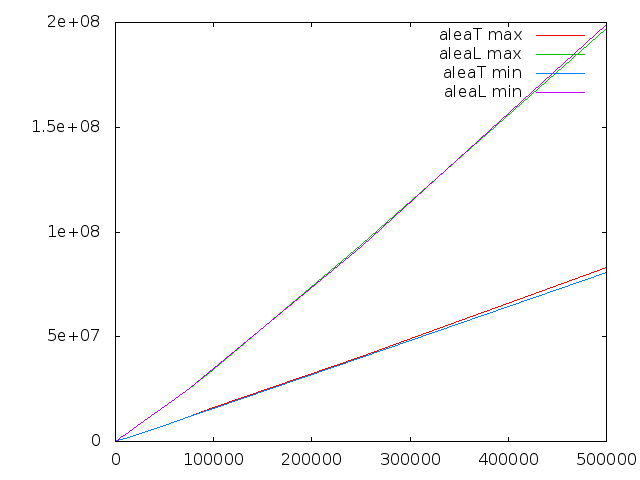
\includegraphics[scale=0.5]{q1.png}
	\caption{les temps d’execution des methodes aleaL et aleaT}
\end{figure}

\section*{Question 2}
Non, on remarque que les courbes min et max de chaque méthodes sont similaires.

\section*{Question 3}
On peut également remarquer que les temps de calcul de l'algorithme aleaL sont plus faible que ceux de aleaT.

\section*{Question 4}
Dans le cas d'un non pseudo aleatoire tout les éléments du tableau ont la même d'être intervertis à la première iteration. Pour les itérations suivantes la probabilitée est la même excepté qu'elle ne peut pas être intervertis avec les itérations précédentes. Mais comme on a montrer qu'a la premiére itération le deuxiéme élément a autant de chance que les autres élément d'étre interverti avec le premier élément par inversion le premiére élément a autant de chance que les autres détre interverti avec le second et donc que chaque permutation des éléments du tableau est équiprobablement obtenue


\newpage


\section*{Question 5}
\begin{figure}[!ht]
	\center
	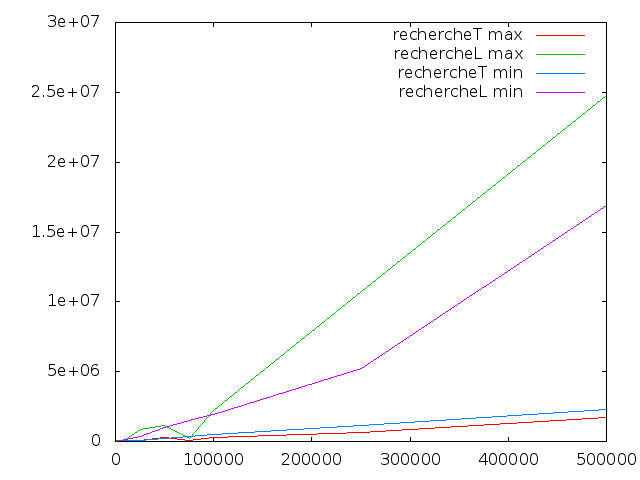
\includegraphics[scale=0.5]{q5.png}
	\caption{les temps d’execution des methodes aleaL et aleaT}
\end{figure}

\section*{Question 6}
Oui la différence est considérable notamment pour l'algorithme rechercheL.

\section*{Question 7}
On remarque que rechercheT max est plus performant que rechercheL min.

\section*{Question 8}
Lorsque le tableau est trié .

\section*{Question 9}
On en conclut que la sélection d'un algorithme doit se faire en fonction du nombre de répetition.

\newpage

\section*{Question 10}
\begin{figure}[!ht]
	\center
	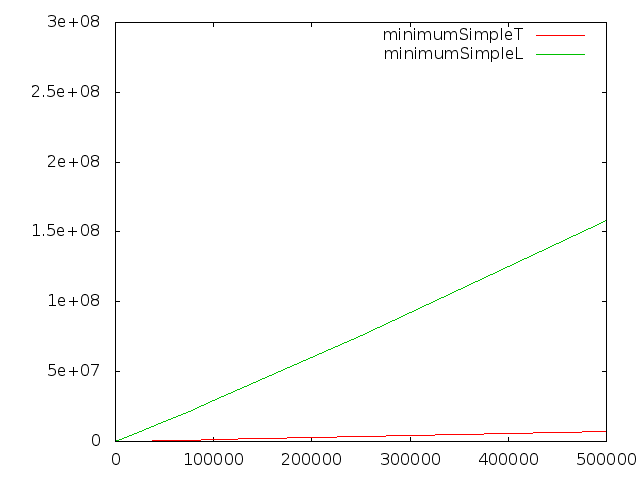
\includegraphics[scale=0.4]{q10.png}
\end{figure}

\section*{Question 11}
\begin{figure}[!ht]
	\center
	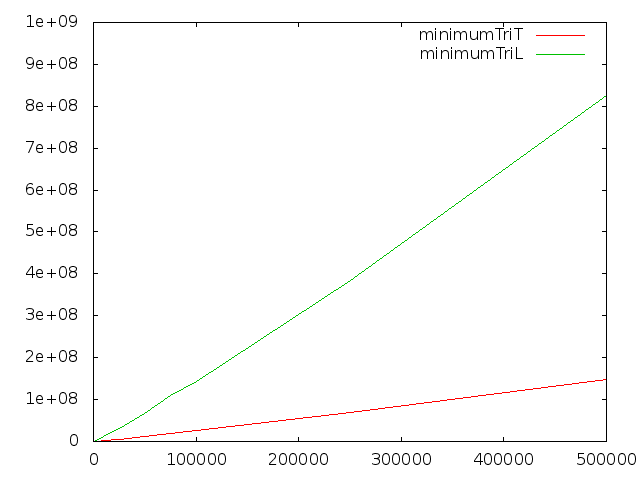
\includegraphics[scale=0.4]{q11.png}
\end{figure}

\section*{Question 12}
Peu importe l'utiltisation le tableau est plus performant que l'arrayList


\newpage
\section*{Question 13}
\begin{figure}[!ht]
	\center
	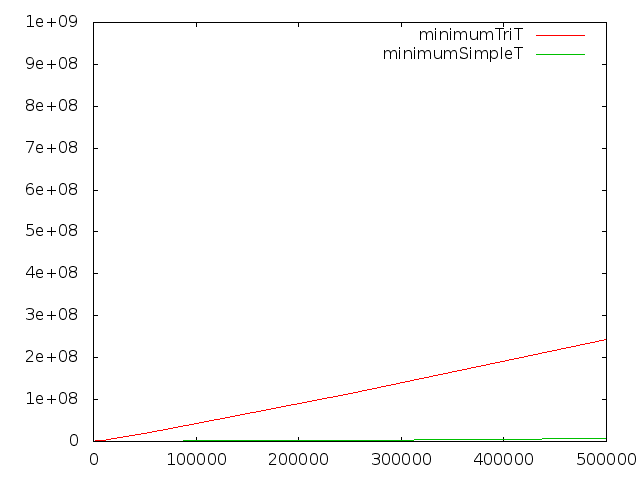
\includegraphics[scale=0.4]{q13.png}
\end{figure}

\section*{Question 14}
\begin{figure}[!ht]
	\center
	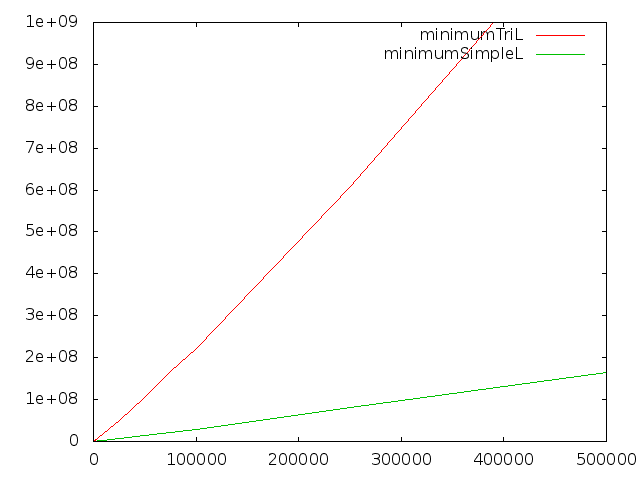
\includegraphics[scale=0.4]{q14.png}
\end{figure}

\section*{Question 15}
Que ce soit une ArrayList ou un tableau, la recherche d'un minima est bien plus performante sans le tri.

\newpage

\section*{Question 16}
\begin{figure}[!ht]
	\center
	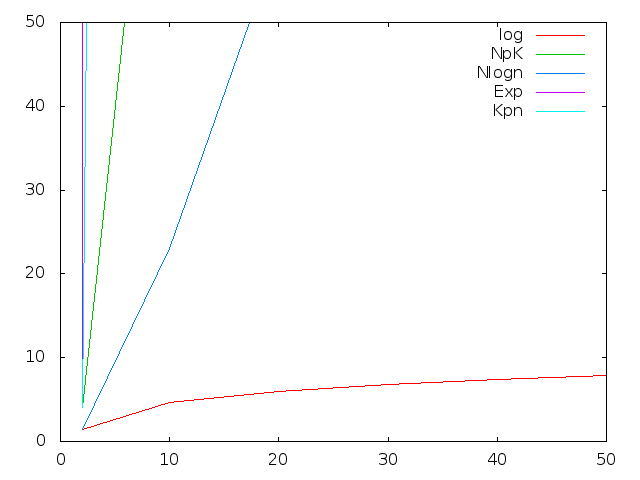
\includegraphics[scale=0.4]{q16.png}
\end{figure}

\newpage

\section*{Question 17}
\begin{figure}[!ht]
	\hbox{ 
     	\hspace*{1cm}
		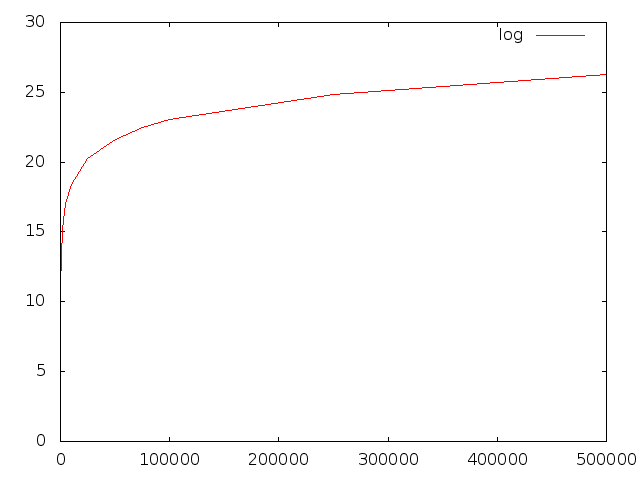
\includegraphics[scale=0.3]{q161.png}
     	\hspace*{1cm}
		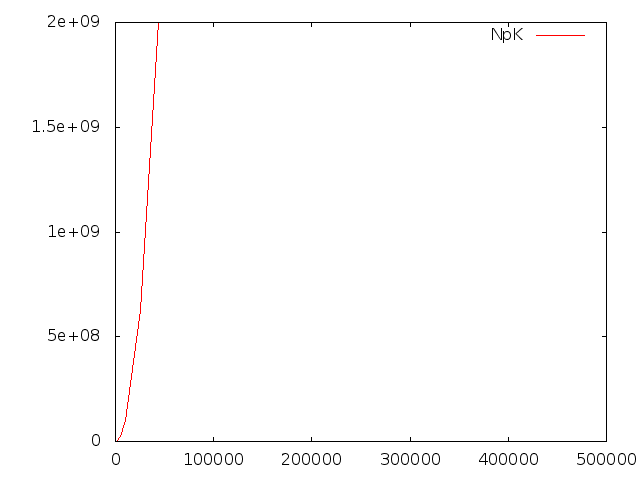
\includegraphics[scale=0.3]{q162.png}
	}
	\hbox{ 
     	\hspace*{1cm}
		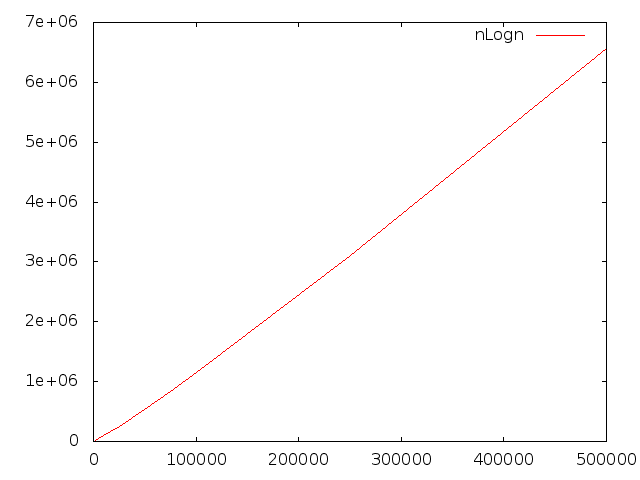
\includegraphics[scale=0.3]{q163.png}
     	\hspace*{1cm}
		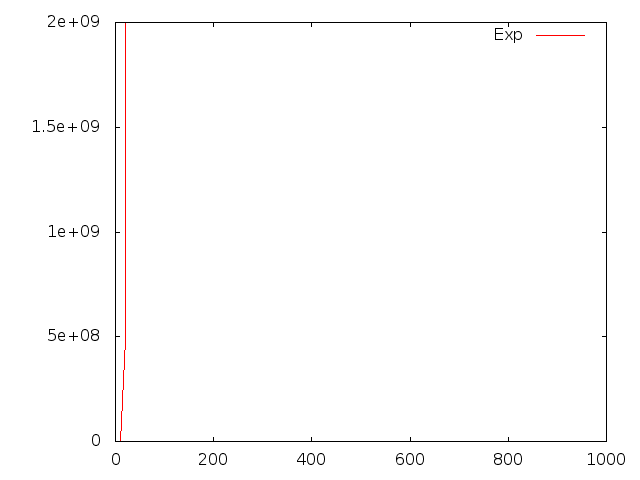
\includegraphics[scale=0.3]{q164.png}
	}
	\hbox{ 
     	\hspace*{5cm}
		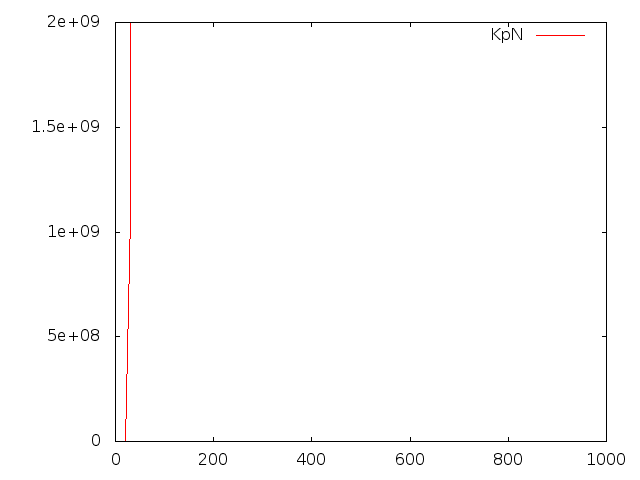
\includegraphics[scale=0.3]{q165.png}
	}
\end{figure}

Comme on peut le voir sur les graphiques ci-dessus, chaque fonction de référence à son ordre de grandeur.
log $\in$ $\mathcal{O}$(nlogn), nlogn $\in$ $\mathcal{O}$(NpK), NpK $\in$ $\mathcal{O}$(KpN), KpN $\in$ $\mathcal{O}$(Exp)

\newpage

\section*{Question 18}
\begin{figure}[!ht]
	\center
	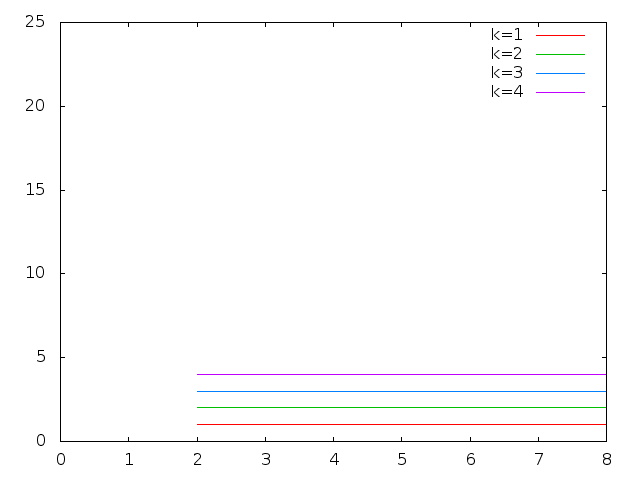
\includegraphics[scale=0.4]{q18.png}
\end{figure}

\section*{Question 19}
log n $\in$ $\Theta$(log n\up{k})
\newpage

\section*{Question 20}
\begin{figure}[!ht]
	\center
	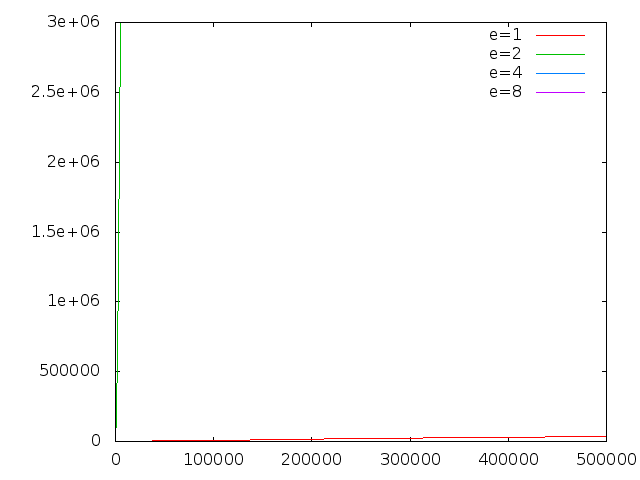
\includegraphics[scale=0.4]{q20.png}
\end{figure}

\section*{Question 21}
\begin{figure}[!ht]
	\center
	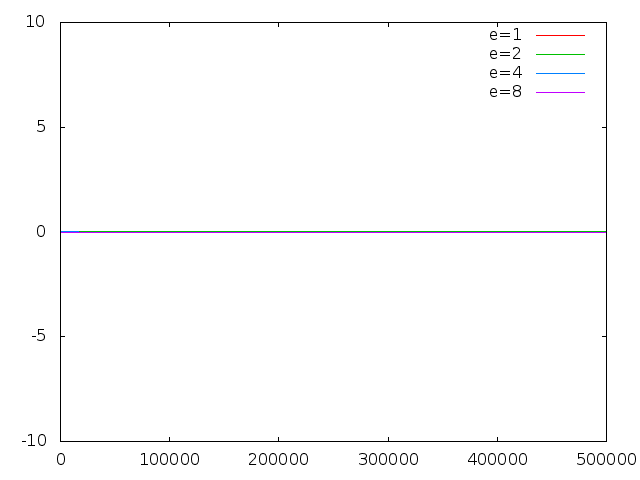
\includegraphics[scale=0.4]{q21.png}
\end{figure}

\section*{Question 22}
log n $\in$ $\mathcal{O}$(n\up{$\varepsilon$})

\newpage

\section*{Question 23}
\begin{figure}[!ht]
	\center
	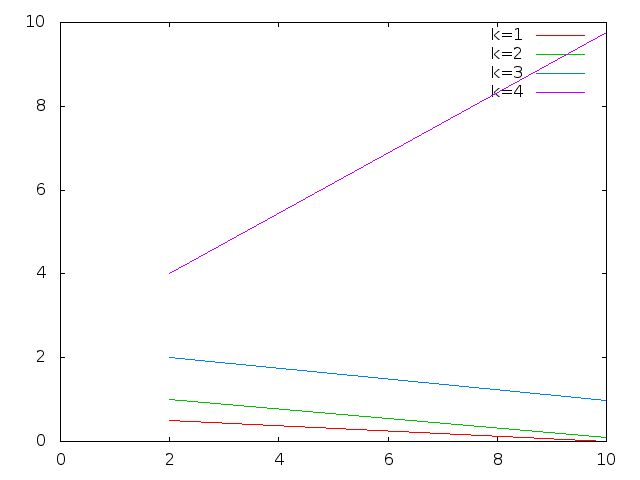
\includegraphics[scale=0.4]{q23.png}
\end{figure}

\section*{Question 24}
\begin{figure}[!ht]
	\center
	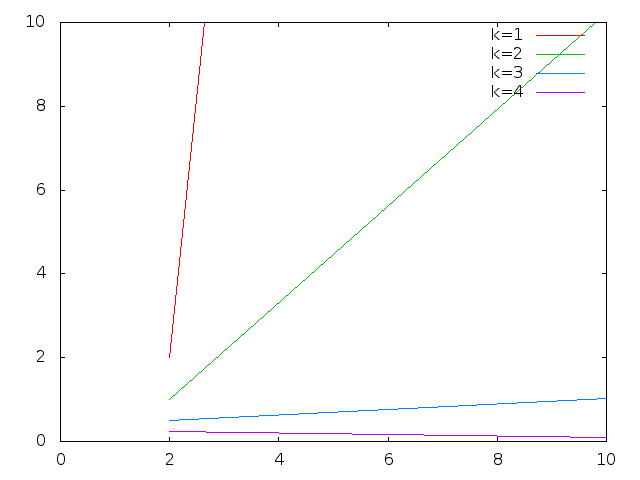
\includegraphics[scale=0.4]{q24.png}
\end{figure}

\section*{Question 25}
2\up{n} $\in$ $\mathcal{O}$(n\up{k})

\newpage

\section*{Question 26}
\begin{figure}[!ht]
	\center
	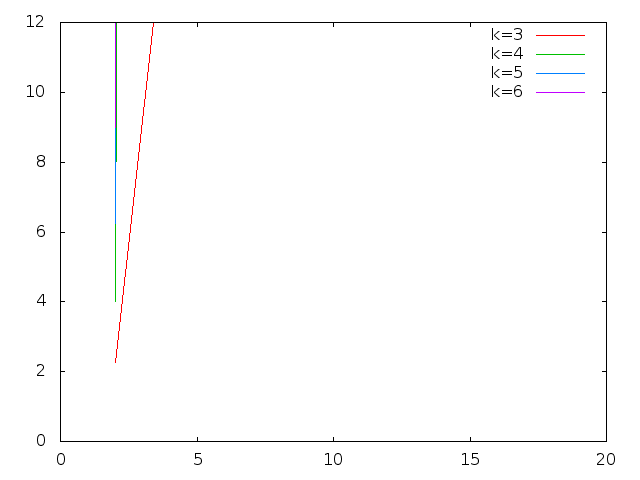
\includegraphics[scale=0.4]{q26.png}
\end{figure}

\section*{Question 27}
\begin{figure}[!ht]
	\center
	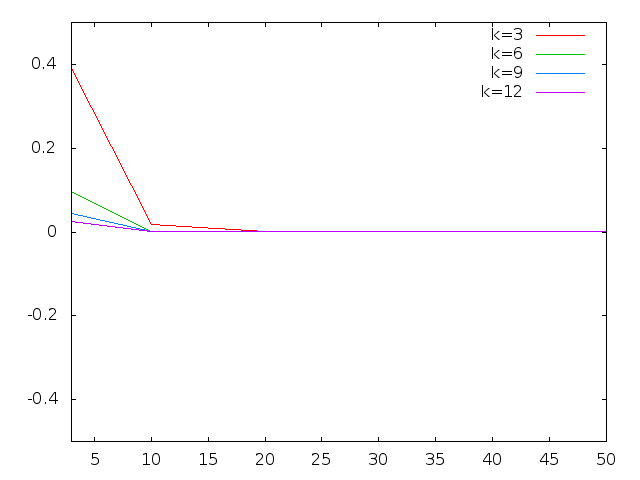
\includegraphics[scale=0.4]{q27.png}
\end{figure}

\section*{Question 28}
2\up{n} $\in$ $\mathcal{O}$(k\up{n})




$\Theta$ $\Omega$
$\mathcal{O}$

\newpage











\end{document}